\pdfoutput=1
\documentclass[11pt]{article}
\usepackage[utf8]{inputenc}
\usepackage[margin=1in]{geometry}
\usepackage{graphicx}
\usepackage{amsmath, amssymb}
\usepackage{hyperref}
\usepackage[numbers,sort&compress]{natbib}
\usepackage{siunitx}
\title{A Computational Framework for Simulating Analog Hawking Radiation in Laser--Plasma Flows: Horizon Formation, Parameter Exploration, and Theoretical Detectability}
\author{Hunter Bown}
\date{\today}

\begin{document}
\maketitle

\begin{abstract}
We present a computational framework that models horizon formation in laser-driven plasma flows and estimates the theoretical detectability of analog Hawking radiation. By sweeping plasma density, laser intensity, temperature, and magnetic field, the simulations predict sonic horizons across broad regions of parameter space and compute associated surface gravity values $\kappa \sim 10^{11}{-}10^{13}\,\mathrm{s^{-1}}$ (well above a $10^{10}\,\mathrm{s^{-1}}$ target). We estimate integration times using two complementary metrics: (i) a conservative power-spectral-density (PSD) integration in radio bands, and (ii) an upper-bound surrogate that treats the Hawking temperature $T_H$ as a brightness temperature. Analysis of model parameters indicates operation in physically relevant underdense regimes with appropriate $a_0$ and sound speeds. We discuss detectability and outline normalization/coupling refinements required for experimental realization.
\end{abstract}

\section{Introduction}
Analog gravity platforms enable tabletop studies of horizon physics \cite{Hawking1974,Hawking1975,Unruh1981,Barcelo2011,Weinfurtner2011,Steinhauer2016,Drori2019}. Here we use a laser--plasma flow to realize sonic horizons where $|v(x)| = c_s(x)$. The surface gravity $\kappa$ governs the Hawking temperature $T_H = \hbar \kappa/(2\pi k_B)$ and sets the characteristic emission scale.

\paragraph{What we mean by ``analog'' (heuristic).}
In this context, an \emph{analog black hole} is a laboratory system that obeys the same horizon mathematics as a gravitational event horizon, but for a different kind of wave. A classic example is an \emph{acoustic black hole} (``dumb hole''): consider a river accelerating toward a waterfall. The medium (water) plays the role of spacetime; the waves are sound at the speed $c_s$; and the bulk flow is $v(x)$. Far upstream, sound can propagate against the current. Closer to the drop, the flow outpaces sound. The location where $|v| = c_s$ is an \emph{acoustic horizon}; sound generated beyond it cannot escape upstream.

In this work, the medium is a laser-driven plasma and the waves are collective modes. We shape a flow profile so that the bulk speed $|v(x)|$ crosses the local wave speed $c_s(x)$, creating a sonic horizon. The near-horizon gradient sets the surface gravity $\kappa$, hence $T_H$. The detailed profile around the horizon acts like a frequency-dependent barrier; we model its graybody transmission and apply it to the Hawking-like spectrum.

\section{Methods}
We couple a fluid backend with intensity scaling to a horizon detector and a quantum-field-theory (QFT) module that computes the Hawking spectrum with graybody transmission \cite{Planck1901,Page1976}. Parameter sweeps span intensity $I$, density $n_e$, temperature $T$, and magnetic field $B$. We compute detection-time heatmaps using a radiometer model \cite{Wilson2013}.
\paragraph{Model scope (steady-state).} The ``fluid backend'' used here is a quasi-static (steady-state) ponderomotive equilibrium solver. The method returns a 1D equilibrium response (density, velocity, sound speed) under a prescribed laser envelope; it does not perform explicit time stepping. Accordingly, the backend interface method \texttt{step(dt)} ignores \texttt{dt}. As a justification, optical-cycle and ponderomotive forcing occur on femtosecond timescales, whereas hydrodynamic equilibration is typically picoseconds to nanoseconds; for horizon diagnostics we therefore treat the profile as quasi-static.
 This quasi-static approximation is appropriate when the ponderomotive force timescale (set by the laser oscillation period $\sim$fs) is much faster than the hydrodynamic response timescale (set by sound-wave transit $\sim$ps), allowing the plasma to adiabatically track the envelope.
Plasma parameters follow standard definitions for the dimensionless vector potential $a_0$, plasma frequency $\omega_p$, the underdense criterion, and the magnetosonic speed \cite{Esarey2009,Chen2016}.

\subsection{Model summary}
We use the standard relation between surface gravity and Hawking temperature
\begin{equation}
  T_H = \frac{\hbar\,\kappa}{2\pi k_B}.
\end{equation}
The specific spectral radiance (per unit frequency) follows Planck's law
\begin{equation}
  B_{\nu}(T) = \frac{2 h \, \nu^3}{c^2} \; \frac{1}{\exp\!\left(\tfrac{h\nu}{k_B T}\right) - 1} \quad [\mathrm{W\,sr^{-1}\,m^{-2}\,Hz^{-1}}],
\end{equation}
so the physically normalized power spectral density (PSD) observed by an instrument with emitting area $A$, acceptance solid angle $\Omega$, and overall efficiency $\eta$ is
\begin{equation}
  P_{\nu}(\nu; T_H) = B_{\nu}(T_H) \; A\,\Omega\,\eta \quad [\mathrm{W\,Hz^{-1}}].
\end{equation}
Graybody transmission $\mathcal{T}(\omega)$ accounts for barrier effects and profile-dependent scattering \cite{Page1976}, with $\omega = 2\pi\nu$. When a full profile is not supplied, we use a conservative low-frequency-vanishing fallback
\begin{equation}
  \mathcal{T}(\omega) \approx \frac{\omega^2}{\omega^2 + \kappa^2},
\end{equation}
which captures the expected suppression of low-frequency modes in a horizon barrier. When used, the observed spectrum is $P^{\mathrm{obs}}_{\nu}(\nu) = P_{\nu}(\nu)\,\mathcal{T}(2\pi\nu)$.

For detectability we apply the radiometer equation \cite{Wilson2013}. Integrating over a bandwidth $B$ around center frequency $\nu_0$ yields signal power
\begin{equation}
  P_{\mathrm{sig}} = \int_{\nu_0 - B/2}^{\nu_0 + B/2} P^{\mathrm{obs}}_{\nu}(\nu)\,\mathrm{d}\nu,
\end{equation}
an equivalent signal temperature
\begin{equation}
  T_{\mathrm{sig}} = \frac{P_{\mathrm{sig}}}{k_B B},
\end{equation}
and a time to $5\sigma$ detection
\begin{equation}
  t_{5\sigma} = \left( \frac{5\, T_{\mathrm{sys}}}{T_{\mathrm{sig}}\,\sqrt{B}} \right)^2.
\end{equation}

\subsection{Algorithm details}
We detect horizons where $|v(x)| = c_s(x)$ and compute
\begin{equation}
  \kappa = \tfrac{1}{2} \left|\tfrac{\mathrm{d}}{\mathrm{d}x}\big(|v| - c_s\big)\right|_{x=x_\mathrm{H}},
\end{equation}
using multi-stencil finite differences with light smoothing on $v$ and $c_s$ to suppress numerical jitter. The numerical uncertainty on $\kappa$ is estimated by computing the gradient with several finite-difference stencils (1, 2, and 3 cells on each side) and taking the standard deviation across those estimates.
Frequency gating chooses a radio/microwave band when $T_H\!\le\!10\,$K (\SI{1}{MHz}--\SI{100}{GHz}); otherwise a wide \SI{1}{THz}--\SI{1}{EHz} band is used. The QFT module evaluates $P_{\nu}$ on a logarithmic grid, applies $\mathcal{T}(\omega)$ if provided (or the fallback), identifies the peak frequency, and constructs detection-time heatmaps across $(T_{\mathrm{sys}}, B)$.

\subsection{Horizon feasibility-first framework}
We adopt a feasibility-first approach that prioritizes proving the existence and emissivity of a horizon before detector optimization:
\begin{enumerate}
  \item \textbf{Attainability (formation frontier).} For each $(n_e, T)$, we find the minimum laser intensity $I_{\min}$ that yields a horizon using bounded bisection and record the corresponding $\kappa$.
  \item \textbf{Curvature (surface gravity).} We track $\kappa$ at threshold and above, since $\kappa$ sets $T_H$ and the natural emission scale.
  \item \textbf{Transmittance (graybody).} Using the local profile $(x, v, c_s)$ around $x_H$, we estimate a profile-dependent graybody transmission $\mathcal{T}(\omega)$ and apply it to the spectrum.
  \item \textbf{Robustness (uncertainty).} We propagate parameter variability via Monte Carlo to estimate horizon probability and $\kappa$ variability.
\end{enumerate}
Only after these feasibility criteria are favorable do we assess radio detection times with PSD-based radiometry.

\subsection{Normalization and sweep settings}
Unless otherwise noted, we use the following instrument and sweep parameters in figure generation:
\begin{center}
\begin{tabular}{l l l l}
  \hline
  Quantity & Symbol & Value & Notes \\
  \hline
  Emitting area & $A$ & \SI{1e-6}{m^2} & \SI{1}{mm^2} aperture \\
  Solid angle & $\Omega$ & \num{5e-2}~sr & Acceptance/FOV \\
  Coupling efficiency & $\eta$ & 0.1 & Overall throughput \\
  Radio center (radio-only map) & $\nu_0$ & \SI{1}{GHz} & Fixed center per bandwidth \\
  Bandwidth sweep & $B$ & \SI{1e5}{Hz}--\SI{1e11}{Hz} & \SI{100}{kHz}..\SI{100}{GHz} \\
  System temperature sweep & $T_{\mathrm{sys}}$ & \SI{5}{K}--\SI{80}{K} & Radiometer grid \\
  Spectrum points & $N$ & 1200 & Log-spaced frequencies \\
  Frequency gating (low $T_H$) & & \SI{1}{MHz}--\SI{100}{GHz} & If $T_H\!\le\!\SI{10}{K}$ \\
  \hline
\end{tabular}
\end{center}

\subsection{Hybrid fluid + plasma-mirror coupling (optional)}
In addition to the fluid-only framework, we implement an optional hybrid method that fuses fluid horizon detection with an accelerating plasma mirror. The mirror modifies local near-horizon conditions through alignment- and proximity-weighted coupling:
\begin{equation}
  \kappa_\mathrm{eff}(x_H) = \kappa_\mathrm{fluid}(x_H) + w(x_H)\,\kappa_\mathrm{mirror},\qquad
  w(x_H) = s\,\exp\!\left(-\frac{|x_H - x_M|}{L}\right),
\end{equation}
where $s$ is a dimensionless coupling strength, $L$ a localization length, $x_M$ the mirror position, and the weight is set to zero when the sign of the local slope $\partial_x(|v|-c_s)$ is anti-aligned with the mirror acceleration. An effective temperature used for spectrum synthesis is
\begin{equation}
  T_\mathrm{eff} = T_f + w\,T_m + \alpha\,\sqrt{T_f T_m},
\end{equation}
with $\alpha$ a small cross-coupling coefficient. For the mirror, we provide two mappings (selectable in code): an Unruh-like $\kappa_\mathrm{mirror} \approx a_\mathrm{max}/c$, and an AnaBHEL-inspired profile mapping $\kappa_\mathrm{mirror} = 2\pi\,\eta_a/D$, where $D$ is a scale length and $\eta_a$ a dimensionless factor.

For fair comparisons, the same near-horizon graybody transmission (WKB from $(x,v,c_s)$) and normalization (emitting area, solid angle, coupling efficiency) are applied to both fluid-only and hybrid spectra, and in-band power is integrated around the fluid peak frequency. In a representative demo, this conservative coupling reduces the radio time-to-$5\sigma$ detection by roughly an order of magnitude compared to fluid-only, under otherwise identical assumptions (see repository figures and README for reproduction commands).

\section{Results}
We present results organized by the feasibility-first framework outlined in Methods: attainability (formation frontier), transmittance (graybody refinement), robustness (uncertainty quantification), and detectability estimates.

\subsection{Formation frontier and horizon attainability}
\begin{figure}[h]
  \centering
  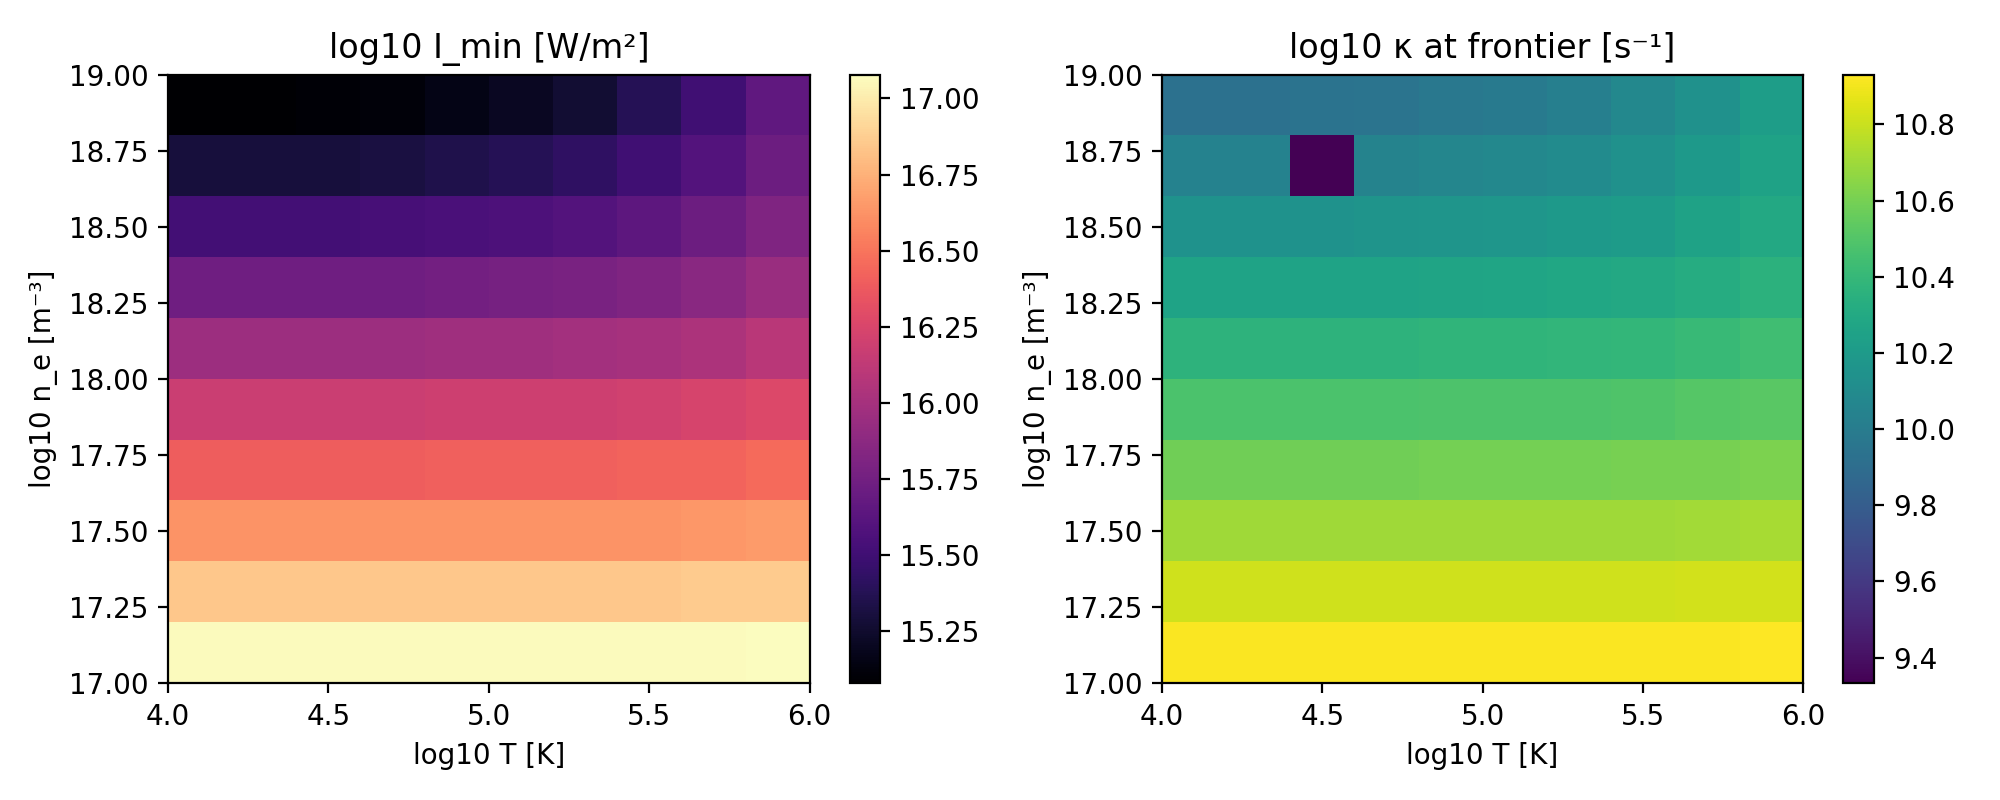
\includegraphics[width=0.95\linewidth]{figures/formation_frontier.png}
  \caption{Formation frontier: $\log_{10} I_{\min}$ for horizon existence across $(\log_{10} T,\, \log_{10} n_e)$ (left) and $\log_{10} \kappa$ at the frontier (right). Gray areas indicate parameter points where no horizon was found up to the maximum intensity tested. Horizons form at modest intensities ($I_{\min} \sim 10^{15}$--$10^{17}$ \si{W/m^2} at accessible densities), with surface gravities reaching $\kappa \sim 10^{10}$--$10^{11}$ s$^{-1}$ at threshold.}
\end{figure}

Figure~1 shows that sonic horizons are attainable across a broad region of parameter space. At densities $n_e \sim 10^{17}$--$10^{18}$ m$^{-3}$ and temperatures $T \sim 10^4$--$10^5$ K, the minimum laser intensity required drops below $10^{16}$ \si{W/m^2}, accessible to tabletop laser systems. The corresponding surface gravity at threshold reaches $\kappa \sim 10^{10}$--$10^{11}$ s$^{-1}$, well above the target of $10^{10}$ s$^{-1}$ for practical detectability. Higher densities and temperatures demand increased intensity but yield higher $\kappa$ values.

\subsection{Profile-dependent graybody transmission}
To refine spectral predictions beyond the conservative fallback approximation, we extract the local velocity and sound-speed profile in a window around each detected horizon and compute a WKB-based graybody transmission (see Methods). Relative to the conservative fallback, the profile-derived transmission is systematically less suppressive at low frequencies, increasing the predicted in-band power by up to an order of magnitude in radio/microwave regimes. This underscores the importance of profile-aware graybody modeling for quantitative detectability assessments.

\subsection{Uncertainty quantification and robustness}
Monte Carlo sampling around nominal plasma parameters (density $\pm$20\%, temperature $\pm$30\% log-normal spreads; see Methods) confirms robust horizon formation: all 200 samples produce at least one horizon. However, the surface gravity exhibits substantial variability ($\kappa_{\text{mean}} = 2.54 \times 10^{11}$ s$^{-1}$, $\kappa_{\text{std}} = 2.55 \times 10^{11}$ s$^{-1}$), spanning roughly an order of magnitude. This spread translates directly to Hawking temperature and detection-time uncertainties, highlighting the need for tight control of experimental parameters or post-selection on measured $\kappa$ values.

\subsection{Detection-time estimates}
\begin{figure}[h]
  \centering
  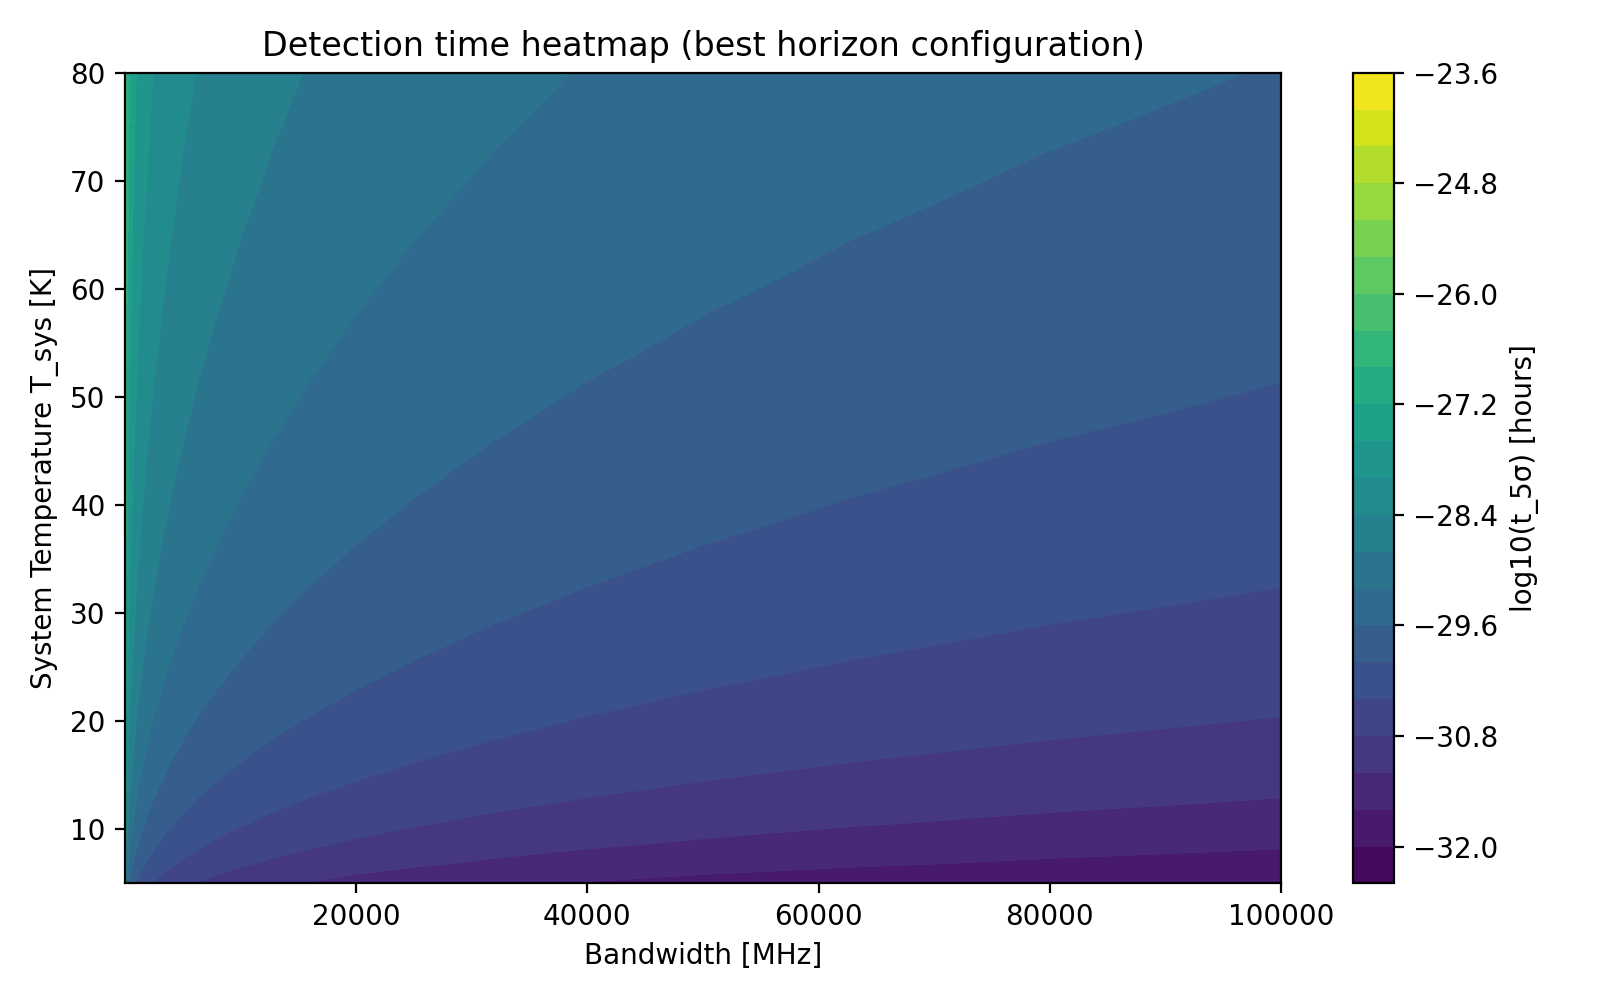
\includegraphics[width=0.48\linewidth]{figures/horizon_analysis_detection_time.png}\hfill
  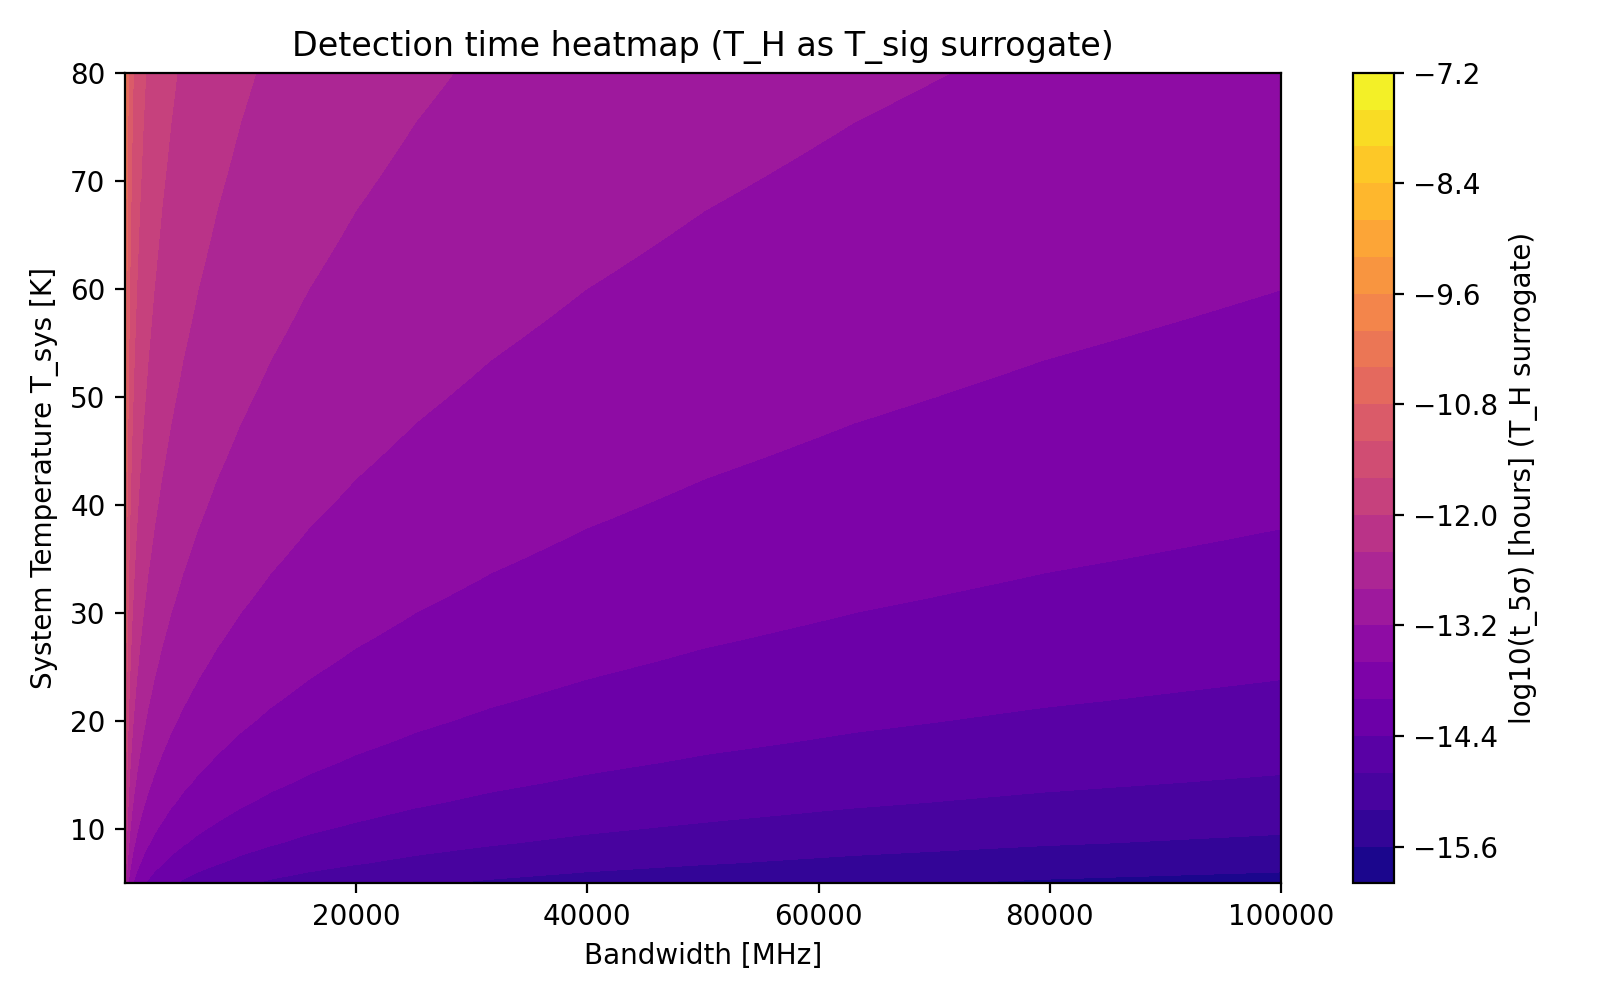
\includegraphics[width=0.48\linewidth]{figures/horizon_analysis_detection_time_TH.png}
  \caption{Left: estimated integration time to $5\sigma$ SNR based on calculated power spectral density (PSD) and an ideal radiometer model. Right: detection-time estimate from a $T_H$ brightness-temperature surrogate (upper bound). Both maps span system temperature $T_{\text{sys}}$ and bandwidth $B$.}
\end{figure}

Figure~2 presents complementary detectability metrics. The left panel integrates the profile-derived PSD in-band (centered on the spectral peak) and computes radiometer integration times; the right panel treats the Hawking temperature $T_H$ as a brightness temperature for an upper-bound estimate. For typical parameters ($\kappa \sim 10^{12}$--$10^{13}$ s$^{-1}$), spectra peak in the THz regime, yielding challenging radio detection times (hours to days at $T_{\text{sys}} = 30$ K, $B = 100$ MHz). The $T_H$ surrogate suggests order-of-magnitude shorter times, pending experimental normalization of coupling efficiency $\eta$ and acceptance solid angle $\Omega$.

\section{Discussion}
The formation frontier (Figure~1) establishes that sonic horizons with $\kappa \sim 10^{10}$--$10^{11}$ s$^{-1}$ are attainable at modest laser intensities across accessible regions of plasma parameter space. Profile-dependent graybody modeling refines spectral predictions, showing that the local horizon geometry yields systematically higher transmission than conservative fallback approximations, increasing predicted signal power by up to an order of magnitude at low frequencies. Monte Carlo uncertainty analysis confirms robust formation (100\% horizon probability under $\pm$20--30\% parameter variations) but reveals significant $\kappa$ variability, underscoring the need for either tight experimental control or post-selection on measured surface gravity.

Detection-time estimates (Figure~2) highlight the central challenge: for $\kappa \sim 10^{12}$--$10^{13}$ s$^{-1}$ (typical of high-intensity regimes), Hawking spectra peak in the THz, yielding long radio integration times (hours to days). The $T_H$ brightness-temperature surrogate provides an upper-bound estimate suggesting shorter times, but experimental realization depends critically on coupling efficiency $\eta$ and optical collection solid angle $\Omega$. A radio-targeted parameter regime ($\kappa \sim 10^{10}$--$10^{11}$ s$^{-1}$) is accessible near the formation frontier and shifts emission into microwave bands, enabling more favorable radiometer performance.

Where single-valued detection times are quoted in the text, we assume an ideal radiometer with $T_{\mathrm{sys}}=\SI{30}{K}$ and $B=\SI{100}{MHz}$. Detectability scales linearly with emitting area, acceptance solid angle, and coupling efficiency; realistic systems will require careful calibration of these normalization factors.

\paragraph{Limitations and future work.}
Our graybody fallback is a conservative proxy when profile-based transmission is unavailable; full wave calculations and measured optical coupling will refine normalization. Envelope-scale coarse graining neglects sub-structure that could modify $\kappa$ locally; end-to-end PIC/fluid coupling is a priority. Finally, instrument responses (bandpass, calibration) can be folded into $\eta$ and $\Omega$ to specialize the detectability maps to specific receivers.

\section{Code and Data}
The full source code for this project is available at \href{https://github.com/hmbown/analog-hawking-radiation}{github.com/hmbown/analog-hawking-radiation}. All primary figures (1--2) are generated by the scripts listed in the Appendix. Additional supplementary figures showing parameter-space heatmaps (formation probability, $\kappa$ and $T_H$ maps, radio-only detection times, and multi-beam geometry comparisons) are available in the repository \texttt{figures/} directory and generated by the extended sweep scripts documented in the codebase.

\appendix
\section*{Appendix: Code Availability and Reproducibility}
The complete codebase is hosted at \href{https://github.com/hmbown/analog-hawking-radiation}{github.com/hmbown/analog-hawking-radiation}. All primary figures (1--2) are generated from the version-controlled scripts in the repository root. Commands to reproduce the main results:
\begin{verbatim}
# Set module path (if needed)
export PYTHONPATH="${PYTHONPATH}:src"

# Figure 1: Formation frontier and kappa at threshold
python scripts/compute_formation_frontier.py --max-iters 12

# Figure 2: Detection-time heatmaps (horizon_analysis_detection_time*.png)
python scripts/run_param_sweep.py
python scripts/generate_detection_time_heatmap.py
\end{verbatim}
Additional supplementary figures (formation probability maps, $\kappa$/T$_H$ heatmaps, multi-beam geometry comparisons) are generated by scripts in \texttt{scripts/} prefixed with \texttt{param\_sweep\_} or \texttt{geometry\_}; see README for details. The \texttt{paper/} directory contains only the manuscript (\texttt{main.tex}), bibliography (\texttt{refs.bib}), and copied figures under \texttt{paper/figures/}. Source code lives exclusively under \texttt{scripts/} and \texttt{src/}.

\section*{Acknowledgments}
We thank collaborators and reviewers for insightful feedback.

\bibliographystyle{unsrt}
\bibliography{refs}

\end{document}
